\documentclass[10pt,openright,twoside,french]{book}

\usepackage{marvosym}
\input philippe2013
\input philippe2013_activites

\pagestyle{empty}

\begin{document}

\TitreExo{1}{\'Etudes de fonctions}

\exo
    \begin{enumerate}
        \item Représenter graphiquement la fonction $x \mapsto \abs x$ pour $x \in \intervalleff{-5}{5}$.
        \item Résoudre graphiquement les équations suivantes :
        \[\abs x = 4 \qq \abs x = 0,5 \qq \abs x = -3\]
        \item Résoudre les inéquations suivantes :
        \[\abs x \leq 2 \qq \abs x > 3 \qq \abs x > -1\]
    \end{enumerate}\[*\]
    
\exo
\begin{minipage}{0.45\linewidth}
    Dans le repère $\left(O \pv \vect\imath, \vect\jmath\right)$ ci-contre, sont représentées trois fonctions dont l'une est une fonction de référence.\par\medskip
    Donner l'expression de $f(x)$, $g(x)$ et $h(x)$ en fonction de $x$.
\end{minipage}\hfill\begin{minipage}{0.45\linewidth}
\begin{center}
    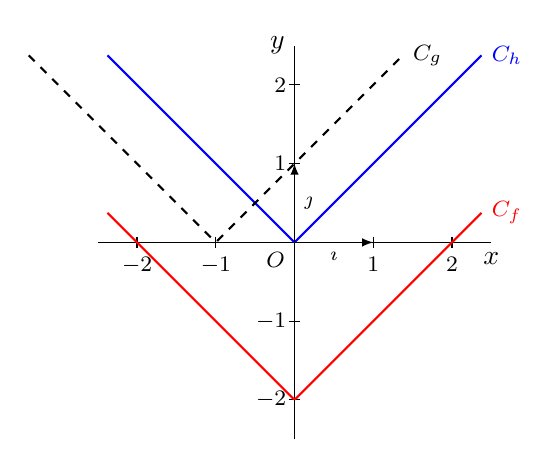
\begin{tikzpicture}[>=latex,x=0.5cm,y=0.5cm]
        \draw (-5,0) -- (5,0) node[below] {$x$} ;
        \foreach \x in {-2, -1,1,2} \draw[xshift=\x cm] (0pt,2pt) -- (0pt,-2pt) node[below] {\footnotesize$\x$};
        \draw (0,-5) -- (0,5) node[left] {$y$} ;
        \foreach \y in {-1,-2,1,2} \draw[yshift=\y cm] (-2pt,0pt) -- (2pt,0pt) node[left=1.5pt] {\footnotesize$\y$};
        \draw (0,0) node[below left] {\footnotesize $O$};
        \draw[blue,thick,domain=-4.75:4.75,samples=200]plot(\x,{abs(\x)}) node[right]{\footnotesize$\calig C_h$};
        \draw[red,thick,domain=-4.75:4.75,samples=200]plot(\x,{abs(\x) - 4}) node[right]{\footnotesize$\calig C_f$};
        \draw[thick,domain=-6.75:2.75,samples=200,dashed]plot(\x,{abs(\x + 2)}) node[right]{\footnotesize$\calig C_g$};
        \draw[->] (0,0) -- (2,0) node[midway,below] {\scriptsize$\vect\imath$};
        \draw[->] (0,0) -- (0,2) node[midway,right] {\scriptsize$\vect\jmath$};
    \end{tikzpicture}
\end{center}
\end{minipage}\[*\]

\exo
Soient $a$, $b$ et $c$ les trois fonctions définies sur $\R$ par :
    \[a(x) = x^2 \qq b(x) = x^2 - 6x + 9 \qetq c(x) = x^2 - 6x + 5\]
\begin{enumerate}
    \item Factoriser l'expression $b(x)$ et écrire la fonction $b$ en fonction de $a$.
    \item \'Ecrire la fonction en fonction de $b$ puis en fonction de $a$.
    \item Par quelle transformation géométrique obtient-on :
        \begin{enumerate}
            \item la courbe de la fonction $b$ par rapport à celle de $a$ ?
            \item la courbe de la fonction $c$ par rapport à celle de $b$ ?
            \item la courbe de la fonction $c$ par rapport à celle de $a$ ?
        \end{enumerate}
    \item Dans un repère orthogonal, tracer les représentations graphiques des fonctions $a$, $c$ et $\abs{c}$.
\end{enumerate}\[*\]

\exo
\begin{minipage}{0.4\linewidth}
La courbe ci-contre représente, dans un repères orthonormal, la tension $u$ en volts en fonction du temps $t$ en secondes.
\begin{enumerate}
    \item En utilisant des fonctions affines, exprimer $u(t)$ en fonction de $t$ sur les intervalles $\intervalleff 0 2$, $\intervalleff 2 4$ et $\intervalleff 4 6$.
    \item On retarde le signal de $1$ seconde, c'est-à-dire qu'on le remplace par la fonction $v$ définie par \[v(t) = u(t + 1).\]
    Représenter graphiquement sur le repère ci-contre la fonction $v$.
\end{enumerate}
\end{minipage}\hfill\begin{minipage}{0.6\linewidth}
\begin{center}
    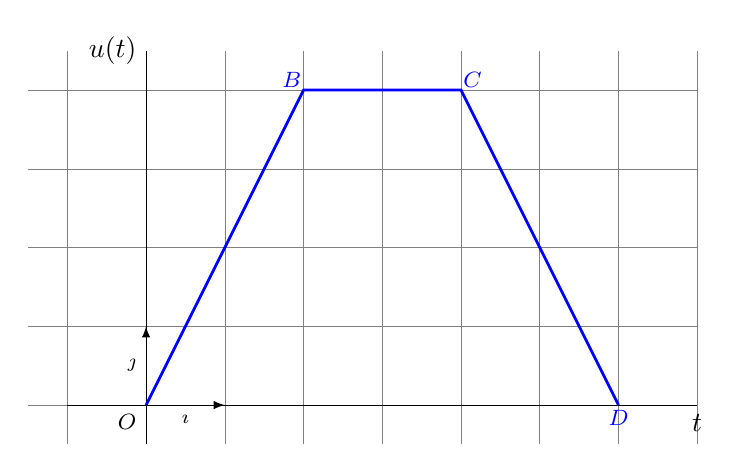
\begin{tikzpicture}[>=latex,x=0.5cm,y=0.5cm]
        \draw[help lines] (-3,-1) grid (14,9);
        \draw (-2,0) -- (14,0) node[below] {$t$} ;
        \draw (0,-1) -- (0,9) node[left] {$u(t)$} ;
        \draw (0,0) node[below left] {\footnotesize $O$};
        \draw[->] (0,0) -- (2,0) node[midway,below] {\scriptsize$\vect\imath$};
        \draw[->] (0,0) -- (0,2) node[midway,left] {\scriptsize$\vect\jmath$};
        \draw[blue,line width = 1pt] (0,0) -- (4,8) node[above left=-3pt] {\footnotesize $B$} -- (8,8) node[above right=-3pt] {\footnotesize $C$} -- (12,0) node [below=-2pt] {\footnotesize $D$};
    \end{tikzpicture}
\end{center}
\end{minipage}

\end{document} 